\documentclass[11pt]{article}

\usepackage[review]{acl}

\usepackage{times}
\usepackage{latexsym}
\usepackage[T1]{fontenc}
\usepackage[utf8]{inputenc}
\usepackage{microtype}
\usepackage{inconsolata}
\usepackage{graphicx}
\usepackage{booktabs}
\usepackage{enumitem}

\title{Causal Evidence on Content-Dependence in Multi-Agent KV-Cache Relay}
% Alternative titles considered (not used):
% - A Causal Audit of KV-Cache Relay Across Chains, Fan-In, and Delegation
% - What Does a Relayed KV Cache Need to Contain? A Causal Audit Across Models and Topologies

\author{Anonymous ACL submission}

\begin{document}
\maketitle

\begin{abstract}
Multi-agent LLM systems increasingly relay key-value (KV) cache between
agents, implicitly treating the cache as transferable state. We test
this with a causal intervention: at the point a cache would be
relayed, we substitute it with (i) the correct, real cache, (ii) an
all-zero cache, (iii) a moment-matched random cache (same per-tensor
mean and standard deviation, no real structure), (iv) a real cache from
a different, unrelated question (\textbf{mismatched}), or (v) no cache
at all (\textbf{dropped}: the receiver gets only its own prompt). We
evaluate this on Qwen2.5-7B-Instruct, Mistral-7B-Instruct-v0.3, and
Qwen3-8B, mostly on HotpotQA, at $n=50$ per condition on a single GPU;
we make no latency claim (chain results for Qwen2.5 and the fan-in are
$n=100$; Mistral and Qwen3-8B remain $n=50$). On Qwen2.5 and Mistral, a
mismatched cache is worse than no relay at all (dropped beats
mismatched, $p<0.0001$ on both) and worse than the correct cache
($p=0.000025$, $p=0.000011$): wrong content actively interferes rather
than merely failing to help. The correct cache is \emph{not} shown to
beat no relay on any model we test ($p=0.68$, $0.29$, $0.42$; the point
estimate's direction differs across models, and Qwen2.5's own estimate
moved toward zero, not away from it, when $n$ doubled) -- not
distinguishable at this sample size, which we do not report as evidence
the cache is unnecessary or that the two are equivalent. On Qwen3-8B we
find no detected sensitivity to cache content at all: mismatched and
dropped produce the identical output string on 45 of 50 examples, while
the correct cache changes roughly 44\% of outputs with no net accuracy
change; we present this as a hypothesis consistent with robustness to
irrelevant context, confounded in this run with non-thinking decoding
mode. A static fan-in decomposition, where the aggregator has no
independent copy of the source passages, shows a different regime:
there the correct cache decisively beats a mismatched one
($p<0.0001$, 30 of 31 discordant pairs), because the cache is its only
route to the evidence rather than one source among several; dropped
beats mismatched there too ($p=0.000076$), the same direction as the
chain, and real vs.\ dropped moved toward significance as $n$ doubled
rather than away from it ($p=0.12\to0.050$, F1 CI excluding zero at
both sizes) -- the opposite trajectory from the chain's own null, which
we read as further evidence for, not just compatible with, the
chain-versus-fan-in distinction below. We adopt
the zeroed/random/mismatched causal-audit methodology
from Cheng et al.\ (2026); our extension is a dropped control, a static
fan-in topology, and a tool-using delegation loop, evaluated under
multi-hop QA and under compression. Compressed relays (8-bit
quantization, a KIVI-inspired 4-bit fix) retain the same
real-versus-mismatched gap as uncompressed relay, so compression does
not turn the cache into interchangeable generic state. We report exact
McNemar tests and bootstrap confidence intervals throughout, with
Holm-adjusted $p$-values for the confirmatory family of comparisons,
and name every comparison that remains underpowered rather than
confirmed.
\end{abstract}

\section{Introduction}

Multi-agent LLM systems increasingly relay key-value (KV) cache between
agents instead of decoded text, to avoid re-encoding information the
receiver would otherwise reprocess. This rests on an assumption that is
rarely tested: that some dimension of the cache, which layer, which
channel, which question's content, can be treated as generic or
interchangeable for compression, reconstruction, or reuse.

We ask directly: can a KV cache produced for one piece of content be
treated as an interchangeable communication artifact, or does it
remain tied to the content that produced it? If a cache carries only
generic transferable state, substituting another valid cache (same
shape, same model, similar statistics) should not systematically change
downstream behavior; if the cache is content-specific, a real cache
from a \emph{different} question should be measurably harmful relative
to the correct one despite being just as valid a tensor, and should be
measurably different from having no cache at all. We operationalize
this with five conditions at the point a cache would be relayed: the
correct \textbf{real} cache; an all-\textbf{zeroed} cache; a
\textbf{moment-matched random} cache (each tensor's own mean/standard
deviation, no real structure); a \textbf{mismatched} cache, real content
from a different held-out question; and \textbf{dropped}, no relayed
cache at all (the receiver's own prompt, unchanged, with nothing
injected in its place). Mismatched and dropped are the most
informative pair: mismatched is not out-of-distribution, it is exactly
as valid a cache as the real one, and dropped isolates whether wrong
content is actively harmful or merely unhelpful by comparing it against
having none. This is an empirical, causal claim about the models,
tasks, and topologies evaluated here ($n=50$ per condition, mostly
HotpotQA, single GPU, no latency claim), not a claim about all KV
caches; we use language such as ``our results indicate'' and ``under
the evaluated models and tasks'' throughout, and name every comparison
that is not statistically significant rather than omit it.

We test this across three topologies and three models. A fixed
sequential three-agent (Reasoner, Verifier, Finalizer) pipeline and a
static fan-in decomposition, where an aggregator receives two parallel
sources instead of one sequential handoff, give structurally different
results once the dropped control is added: in the chain, the receiver
already has the source passages in its own prompt, so a wrong cache
acts as interference and dropped scores close to the real cache; in
the fan-in, the aggregator has no such independent copy, so the cache
is its only route to the evidence and the correct cache decisively
beats a mismatched one. A dynamic, model-driven delegation loop in the
style of Recursive Language Models (RLMs) \citep{rlm2026}, where the
root model itself decides turn by turn what to delegate, shows the
causal audit still resolves there even on a final-answer accuracy
comparison it cannot itself resolve. Across Qwen2.5-7B-Instruct and
Mistral-7B-Instruct-v0.3, mismatched content is consistently worse than
both the correct cache and no cache at all; on Qwen3-8B, evaluated in
non-thinking mode, we detect no sensitivity to cache content at all,
and we do not claim to know whether this is an architecture effect, a
decoding-mode effect, or both. Building on this, we test KV-relay
efficiency techniques and find compression that does not disturb this
same real-versus-mismatched gap.

This paper makes three contributions. \textbf{(1) A dropped (no-relay)
control added to an existing causal-audit methodology}: on two of three
models, a mismatched cache is shown worse than no cache at all, not
only worse than the correct one, which a zeroed/random/mismatched-only
design cannot show. \textbf{(2) Two structurally different regimes
identified, not conflated}: a sequential chain where the receiver has
an independent information path, and a fan-in where it does not, with
the dropped control behaving differently in each for a stated reason
tied to topology, not model. We also report, rather than omit, a model
(Qwen3-8B) where we detect no cache-content sensitivity at all.
\textbf{(3) Compression evaluated under the same causal lens}: the
compressed relays we test retain the real-versus-mismatched gap,
evidence against compression silently turning the cache into generic
state, alongside techniques that fail for reasons the causal audit
itself helps explain.

\section{Related Work}
\label{sec:related}

Relaying KV cache instead of text has been proposed to avoid redundant
prefill. KVCOMM \citep{kvcomm2025} corrects KV-cache offset drift when
reusing cache across prefixes; LatentMAS \citep{latentmas2026} exchanges
autoregressive latent ``thoughts'' via KV working memory. We differ by
relaying real decoded reasoning through a fixed three-agent chain on
multi-hop QA \citep{hotpotqa2018}, which neither tested. For
compression we adopt layer-wise selection (dropping calibration-
identified low-importance layers, reconstructed via \texttt{zeros},
\texttt{nearest}, or \texttt{interpolate}) and per-head quantization;
Orthogonal Backfill \citep{orthobackfill2026} and KVTC \citep{kvtc2026}
are related strategies we considered but did not adopt (Appendix
\ref{app:relwork}). A rotation-based scheme in the style of TurboQuant
\citep{turboquant2026} and PolarQuant \citep{polarquant2026} produced
severely out-of-distribution output on our pipeline; we traced this to
keys' rotary position embeddings (RoPE), cached post-rotation, being
disrupted by a second, RoPE-agnostic rotation (full diagnostic in
Appendix~\ref{app:rotation}). KIVI \citep{kivi2024}, RotateKV
\citep{rotatekv2025}, and KVQuant \citep{kvquant2024} independently
identify this post-RoPE key sensitivity; our KIVI-inspired per-channel
fix confirms it directly, resolving \texttt{B\_int4}'s collapse to
52.0\%/64.1\% F1 at 3.96x compression (Section~\ref{sec:results}).

Cheng et al.\ \citep{latentcommpay2026} audit relayed KV cache with
deranged (mismatched), zeroed, and moment-matched random substitution
across three model families and five checkpoints, showing that a
mismatched-cache control is necessary to credit downstream gains to
content rather than to the mere presence of a non-empty cache; our
zeroed/random/mismatched methodology follows this framework rather than
introducing it. Zhang and Emu \citep{zhangemu2026} independently apply a
closely related causal-audit methodology to latent relay on
Qwen3-4B/8B. Our contribution relative to both is the conditions and
topologies we add: a \textbf{dropped} control (the receiver gets only
its own prompt, with no relayed cache at all, distinct from a zeroed or
substituted one), a static fan-in decomposition and a tool-using
delegation loop in addition to a fixed sequential chain, multi-hop QA,
and compressed as well as uncompressed relays. Concretely, this is not
simply broader coverage: a zeroed/random/mismatched-only design always
relays \emph{something}, so it cannot distinguish a receiver actively
misled by wrong content from one merely deprived of right content. The
dropped control answers exactly that question, and the answer is not
trivial: on Qwen2.5 and Mistral, wrong content is shown significantly
worse than no content at all ($p<0.001$; Section~\ref{sec:results}), a
distinction neither prior design is built to draw. Cheng et al.'s own
headline finding, that content-specificity is system-dependent, and our
own Qwen3-8B exception (Section~\ref{sec:results}) converge on the same
qualitative pattern from different varied axes
(Appendix~\ref{app:relwork}).

Brito and Baquero \citep{latentagentslie2026} audit KV-cache integrity
under an adversarial specialist agent that visibly commits to one
message while passing a manipulated hidden cache state, a threat-model
variant of the same substitution question we ask under a
non-adversarial, measurement-only framing. Recursive Language Models
\citep{rlm2026} let a root model delegate via a sandboxed Python REPL
rather than a fixed topology; LatentMAS \citep{latentmas2026} and
CanonicalMerge \citep{canonicalmerge2026} (Baquero and Brito) relay
richer-than-text content but over a topology still fixed by the system
designer. CanonicalMerge is close to our fan-in topology (near-identical
models and task) but tests only downstream accuracy, not causal
necessity of content. To our knowledge no prior work tests whether
relayed content is causally necessary once delegation is no longer
fixed by the designer. Li, An, and Du's Orthogonal Backfill
\citep{orthobackfill2026} compresses relayed latent content by
injecting a low-rank residual of discarded content rather than
discarding it outright; we consider but do not adopt it
(Section~\ref{sec:method}, Appendix~\ref{app:relwork}). \texttt{KVCOMM}
\citep{kvcomm2025} (Ye et al., introduced above) and \texttt{KVComm}
\citep{shikvcomm2025} (Shi et al.) are distinct papers despite the
near-identical name; we do not otherwise discuss the latter here.

``No Free Swap'' \citep{nofreeswap2026} finds layer interchangeability
is model- and protocol-dependent, consistent with our own
architecture-dependent layer-selection cost. ``Rethinking Layer
Redundancy'' \citep{rethinkredundancy2026} raises exactly the question
we test directly in Section~\ref{sec:results}: whether a calibration
signal's own confidence predicts safety. It does not, and fails in the
wrong direction. AdaK \citep{adak2026} and ``The Pitfalls of KV Cache
Compression'' \citep{pitfallskv2026} are discussed in
Appendix~\ref{app:relwork}; our contribution relative to both is a
causally grounded, cross-axis demonstration within one system rather
than an aggregate-metric or single-axis argument.

\section{Method}
\label{sec:method}

\paragraph{Why these pipelines are built from scratch.} No
general-purpose multi-agent orchestration framework we are aware of
(LangGraph, AutoGen, CrewAI, DSPy) exposes KV cache as an inter-agent
channel; each treats an agent's output as decoded text or a structured
message, with the model's internal cache a private implementation
detail the framework never surfaces. Testing whether relayed KV is
causally necessary therefore requires building the relay mechanism
directly on the model's own cache API in every topology below, not
adapting an existing agent framework (we verified this specifically for
the delegation loop against DSPy's own documentation before committing
to a from-scratch implementation; Appendix~\ref{app:method-ext}). The
three pipelines that follow are deliberately minimal for this reason:
built to isolate the causal question under test, not to match a
published system's scale or task coverage.

\paragraph{Pipeline and models.} We study a sequential three-agent
pipeline (Reasoner, Verifier, Finalizer) on HotpotQA
\citep{hotpotqa2018} (distractor configuration, ten candidate passages
per item); a GSM8K \citep{gsm8k2021} run confirms generalization.
\texttt{text\_agent} passes decoded text between agents;
\texttt{A}--\texttt{E} relay KV cache directly; \texttt{single\_agent}
is a no-relay control. All share identical prompts, so accuracy/latency
deltas are attributable to the relay mechanism itself. We evaluate
Qwen2.5-7B-Instruct \citep{qwen2p5_2024} (bf16, primary) and
Mistral-7B-Instruct-v0.3 \citep{mistral7b2023} (bf16, architectural
diversity at comparable scale) on the full configuration suite, and
Qwen3-8B (bf16) on \texttt{A}/\texttt{D} only ($n=50$) to extend the
architecture-dependence check to a third point. Phi-3.5-mini-instruct
was evaluated and dropped after isolating a pre-existing LongRoPE
limitation unrelated to our pipeline (Appendix~\ref{app:limitations}).

\paragraph{Configurations.} \texttt{B\_int8}/\texttt{B\_int4} apply
uniform per-head min-max quantization. \texttt{C} drops
calibration-identified low-importance layers. \texttt{D} combines
layer selection with adaptive per-tier quantization (8-bit/4-bit).
\texttt{E} adds an anchor-based offset-correction mechanism adapted
from KVCOMM. \texttt{B\_int4\_kivi} fixes \texttt{B\_int4}'s collapse by
quantizing keys per-channel instead of per-head (Section
\ref{sec:results}).

\paragraph{Causal audit.} At the point a KV cache would be relayed, we
substitute (i) an all-zero cache, (ii) a moment-matched random cache,
(iii) a held-out question's real cache (\textbf{mismatched}), or (iv)
no cache at all (\textbf{dropped}: the receiver's own prompt is sent
unchanged, but \texttt{past\_key\_values} is never populated for that
hop, not set to a zeroed or substituted tensor), applied to our three
strongest chain configurations (\texttt{A}, \texttt{B\_int8},
\texttt{D}) and to the fan-in's \texttt{kv} condition. Mismatched donor
caches are drawn from a pool of 20 held-out questions never among the
scored set, confirmed non-overlapping by direct question-text
comparison; each scored example draws one donor assignment, not
resampled across conditions. We treat zero-ablation as a known-
imperfect, out-of-distribution baseline and the random/mismatched/
dropped conditions as the more informative evidence (Appendix
\ref{app:method-ext}). Table~\ref{tab:conditions} summarizes what the
receiver's own context contains under each condition.

\begin{table}[t]
\centering
\small
\begin{tabular}{lp{3.5cm}p{3.1cm}}
\toprule
\textbf{Condition} & \textbf{Chain (Verifier/Finalizer)} & \textbf{Fan-in (aggregator)} \\
\midrule
real & own prompt + real upstream KV & own prompt + both children's real KV \\
dropped & own prompt only, no KV & own prompt only, no KV \\
zeroed & own prompt + all-zero KV & own prompt + all-zero children's KV \\
random & own prompt + moment-matched noise KV & own prompt + moment-matched noise KV \\
mismatched & own prompt + a different question's real KV & own prompt + a different question's children's real KV \\
\bottomrule
\end{tabular}
\caption{What the receiver's context contains under each causal-audit
condition. In both topologies the receiver's own prompt text asserts
that prior content is already in context (the Verifier/Finalizer
prompts in the chain, the aggregator prompt in the fan-in); this
assertion is false under \textbf{dropped}. We left these prompts
identical across all five conditions so that only the cache differs
between them, at the cost of that assertion being literally false in
exactly the dropped condition (Limitations).}
\label{tab:conditions}
\end{table}

\paragraph{Fan-in and RLM+KV topologies.} In the fan-in topology,
HotpotQA's ten passages are split across two child agents; their
RoPE-shifted caches are concatenated before one aggregator attends over
both. The audit substitutes every child's KV, not one while leaving the
other as an unaudited shortcut (an early design bug we fixed; Appendix
\ref{app:faninbug}). In the RLM+KV topology, a root model writes and
executes code in a sandboxed Python REPL, deciding what to delegate and
when, until it calls \texttt{final\_answer(...)}; we implement two
sub-call return channels, \texttt{text} (RLM's own mechanism) and
\texttt{kv} (the sub-call's real cache is RoPE-shifted and spliced onto
the root's running cache instead), so the two differ only in what is
relayed. The audit substitutes a sub-call's real KV identically to the
fixed topologies. Unlike both fixed topologies, the root retains direct
access to the original passages independent of any sub-call, so
corrupting one sub-call's KV does not remove all of the root's
information (Section~\ref{sec:results}, Limitations). We implement this
from scratch on \texttt{transformers} \citep{transformers2020} rather
than \texttt{dspy.RLM}, which exposes no KV access (Appendix
\ref{app:method-ext}).

\paragraph{Statistics.} For headline comparisons we report exact
McNemar's test on paired per-example correctness and a paired bootstrap
95\% CI (10,000 resamples) for mean F1 difference, plus Monte Carlo
power for non-significant comparisons. Every $p$-value reported in this
paper is \textbf{uncorrected} for multiple comparisons unless stated
otherwise. We designate one \textbf{confirmatory family}:
real-vs-mismatched and dropped-vs-mismatched, per model and topology
(Table~\ref{tab:no_relay}), the comparisons headline claim 1 rests on.
Holm-adjusted $p$-values for all 8 members of this family
(Table~\ref{tab:no_relay}; Qwen2.5 chain and fan-in at $n=100$, Mistral
and Qwen3-8B at $n=50$): Qwen2.5 fan-in real-vs-mismatched
$3.0\times10^{-8} \to 2.4\times10^{-7}$; Qwen2.5 chain
dropped-vs-mismatched $6.9\times10^{-8} \to 4.9\times10^{-7}$; Mistral
chain real-vs-mismatched $1.1\times10^{-5} \to 6.6\times10^{-5}$;
Qwen2.5 chain real-vs-mismatched $2.5\times10^{-5} \to 1.3\times10^{-4}$;
Qwen2.5 fan-in dropped-vs-mismatched $7.6\times10^{-5} \to
3.0\times10^{-4}$; Mistral chain dropped-vs-mismatched $4\times10^{-4}
\to 1.2\times10^{-3}$; Qwen3-8B chain real-vs-mismatched $0.30 \to
0.60$; Qwen3-8B chain dropped-vs-mismatched $1.0 \to 1.0$. Every family
member significant before correction remains significant after it, and
the two members rerun at higher $n$ (Qwen2.5 chain and fan-in
dropped-vs-mismatched) strengthened rather than weakened under added
power. Every other comparison in this paper (zeroed/random legs,
cross-model layer-selection costs, compression comparisons) is
\textbf{descriptive}: reported with its own exact $p$-value and CI, not
part of a pre-registered confirmatory family.

\section{Results}
\label{sec:results}

We present results in the order the argument is built: causal evidence
on the simplest topology (\S\ref{sec:results}.1), its generalization
across topology and architecture (\S\ref{sec:results}.2--.3), then its
implications for compression (\S\ref{sec:results}.4). Unless noted,
figures are accuracy/F1 (\%).

% Consolidated causal-audit table -- draft for review before insertion into main.tex.
% Covers every real/zeroed/random/mismatched comparison currently spread
% across six "Finding 5, extended..." paragraphs, plus the new topology
% generalization rows (fan-in, RLM+KV) not yet in main.tex.

\begin{table*}[t]
\centering
\small
\begin{tabular}{llcccccc}
\toprule
\textbf{Config} & \textbf{Model / Task / Topology} & \textbf{Real} & \textbf{Zeroed} & \textbf{Random} & \textbf{Mismatched} & \textbf{$n$} \\
\midrule
\multicolumn{7}{l}{\emph{Qwen2.5-7B-Instruct, HotpotQA, sequential chain}} \\
A            & --                          & 50.0/64.0 & 0.0/0.0  & 0.0/0.0  & 28.0/37.1 & 50 \\
D            & --                          & 54.0/60.2 & 0.0/0.0  & 0.0/0.2  & 26.0/32.2 & 50 \\
B\_int8      & --                          & 54.0/68.0 & 0.0/0.0  & 0.0/0.0  & 24.0/34.4 & 50 \\
C            & --                          & 46.0/55.7 & 0.0/0.0  & 0.0/0.0  & 24.0/38.9 & 50 \\
B\_int4\_kivi& --                          & 50.0/61.7 & 0.0/0.0  & 0.0/0.0  & 28.0/34.7 & 50 \\
\midrule
\multicolumn{7}{l}{\emph{Generalization: model, task, and topology}} \\
A            & Mistral-7B-Instruct-v0.3    & 56.0/63.3 & 0.0/0.5  & 0.0/0.3  & 16.0/26.4 & 50 \\
C            & Mistral-7B-Instruct-v0.3    & 20.0/30.3 & 0.0/0.5  & 0.0/0.1  & 14.0/26.1 & 50 \\
D            & Mistral-7B-Instruct-v0.3    & 22.0/32.8 & 0.0/0.5  & 0.0/0.1  & 16.0/29.3 & 50 \\
B\_int8      & Mistral-7B-Instruct-v0.3    & 56.0/63.3 & 0.0/0.5  & 0.0/0.1  & 20.0/29.3 & 50 \\
B\_int4\_kivi& Mistral-7B-Instruct-v0.3    & 54.0/63.2 & 0.0/0.5  & 0.0/0.1  & 16.0/25.0 & 50 \\
A            & Qwen3-8B                    & 54.0/67.2 & 46.0/55.8& 0.0/0.0  & 64.0/74.8 & 50 \\
D            & Qwen3-8B                    & 56.0/71.2 & 46.0/55.8& 2.0/5.0  & 52.0/62.4 & 50 \\
A            & GSM8K (Qwen2.5)             & 90.0/---  & 0.0/---  & 2.0/---  & 28.0/---  & 50 \\
A            & 2WikiMultihopQA (Qwen2.5)   & 54.0/62.5 & 0.0/0.7  & 0.0/0.0  & 16.0/23.4 & 50 \\
kv (fan-in)  & Fan-in topology (Qwen2.5)   & 40.0/53.0 & 0.0/0.8  & 0.0/0.0  & 6.0/12.0  & 50 \\
kv (RLM+KV)  & Dynamic delegation (Qwen2.5)& 24.0/32.3 & 8.0/11.2 & 6.0/9.2  & 10.0/15.5 & 50 \\
\bottomrule
\end{tabular}
\caption{Every real/zeroed/random/mismatched causal-audit comparison in this
paper: accuracy/F1 (\%) per condition. \emph{Real} vs.\ \emph{zeroed}/\emph{random}
is significant ($p<0.0001$) in every row except Qwen3-8B, where content-dependence
itself is architecture-dependent (see text). \emph{Real} vs.\ \emph{mismatched}
is significant in all rows except Mistral \texttt{C}/\texttt{D} (underpowered on
an already-degraded layer-selection baseline, see Finding 3) and Qwen3-8B (a
distinct, architecture-dependent finding, see text). GSM8K reports accuracy only
(no partial-credit F1 metric for this task).}
\label{tab:causal_audit_full}
\end{table*}


\subsection{Sequential relay: KV content is causally relevant}

On \texttt{A} ($n=50$): 50.0/64.0 real versus 0.0/0.0 zeroed and random
versus 28.0/37.1 mismatched. Every comparison is significant (real
vs.\ zeroed/random $p<0.0001$ each; real vs.\ mismatched $p=0.0127$;
mismatched vs.\ zeroed/random $p=0.0001$). This underwrites every
compression result below: they are only meaningful claims about
preserved information if relay carries real content in the first
place. Table~\ref{tab:causal_audit_full}
extends this to \texttt{D}, \texttt{B\_int8}, \texttt{C},
\texttt{B\_int4\_kivi} (same ordering: real vs.\ zeroed/random
$p<0.0001$ throughout, real vs.\ mismatched $p=0.0013$--$0.0192$,
mismatched vs.\ zeroed/random $p=0.0001$--$0.0005$, tighter than
\texttt{A}'s own), a GSM8K confirmatory run (same ordering, more
decisive), and both generalization axes below.

% No-relay (dropped) causal-audit control, added against the real/mismatched
% ladder already in table_causal_audit_full.tex. Qwen2.5 chain and Qwen2.5
% fan-in rows are n=100 (rerun 2026-10-09 to add power to the two weakest
% legs, results/run_20261009_113254 and
% results/recursive_poc_check/run_20261009_125426); Mistral and Qwen3-8B
% rows remain n=50 (not rerun). Paired exact McNemar throughout.

\begin{table*}[t]
\centering
\small
\begin{tabular}{lccccccc}
\toprule
\textbf{Model / Topology} & \textbf{Real} & \textbf{Dropped} & \textbf{Mismatched} & \textbf{$p$(Real,Dropped)} & \textbf{$p$(Real,Mismatched)} & \textbf{$p$(Dropped,Mismatched)} & \textbf{$n$} \\
\midrule
Qwen2.5-7B-Instruct chain          & 56.0/69.1 & 59.0/69.0 & 29.0/40.6 & 0.68   & 0.000025 & $<0.0001$ & 100 \\
Mistral-7B-Instruct-v0.3 chain     & 56.0/63.3 & 48.0/58.4 & 16.0/26.4 & 0.29   & 0.000011 & 0.0004   & 50 \\
Qwen3-8B chain$^\dagger$           & 54.0/67.2 & 62.0/71.4 & 64.0/74.8 & 0.42   & 0.30     & 1.0      & 50 \\
Qwen2.5-7B-Instruct fan-in         & 37.0/46.6 & 25.0/33.4 & 8.0/13.0 & 0.050  & $<0.0001$ & 0.000076 & 100 \\
\bottomrule
\end{tabular}
\caption{No-relay (\textbf{dropped}: receiver gets only its own prompt, no
relayed cache) added to the real/mismatched comparison. Accuracy/F1 (\%) per
condition; $p$-values are exact paired McNemar, uncorrected (Section~\ref{sec:results}
gives the Holm-adjusted values for the confirmatory family). $^\dagger$Qwen3-8B
ran with \texttt{enable\_thinking=False} (non-thinking mode); we cannot
separate an architecture effect from a decoding-mode effect from this run
alone. Qwen2.5 chain and fan-in are $n=100$ (Mistral and Qwen3-8B remain
$n=50$): doubling $n$ pulled the chain's real-vs-dropped point estimate
toward zero (56.0\% vs.\ 59.0\%, F1 diff $+0.1$ pts, 95\% CI $[-8.2,
+8.4]$) while the fan-in's moved the other way, toward significance
($p=0.12\to0.050$, F1 diff $+13.2$ pts, 95\% CI $[+2.2, +24.2]$) --
opposite trajectories under added power, consistent with (not just
compatible with) the chain-vs-fan-in mechanism in \S\ref{sec:results}.1.
Note: Table~\ref{tab:causal_audit_full}'s \texttt{A} and fan-in
\texttt{kv} rows report the original $n=50$ zeroed/random/mismatched
ladder; this table's Qwen2.5 real/mismatched figures come from the
separate, later $n=100$ rerun above, which did not re-run
zeroed/random -- the two tables' numbers for the same-named config
differ by design, not by error.}
\label{tab:no_relay}
\end{table*}


Adding a \textbf{dropped} control (Table~\ref{tab:no_relay};
Section~\ref{sec:method}: the receiver gets only its own prompt, no
relayed cache at all) sharpens this picture and narrows one claim we
can make. On both Qwen2.5 and Mistral, a mismatched real cache is worse
than no relay at all (dropped beats mismatched, $p<0.001$ on both:
$p<0.0001$, $p=0.0004$) and worse than the correct cache
($p=0.000025$, $p=0.000011$): wrong content is not merely unhelpful, it
is actively worse than having none. The same direction holds in the
fan-in topology as well (dropped beats mismatched, $p=0.000076$, 18 of
19 discordant pairs favoring dropped; \S\ref{sec:results}.2), so this
is not specific to the chain. We do \emph{not}, however, find
that the correct cache beats no relay on any model in the chain:
\texttt{A} vs.\ dropped is not significant on Qwen2.5 ($p=0.68$,
$n=100$), Mistral ($p=0.29$, $n=50$), or Qwen3-8B ($p=0.42$, $n=50$),
and the point estimate's direction is inconsistent across models
(dropped numerically ahead on Qwen2.5 and Qwen3-8B; real ahead on
Mistral). Doubling Qwen2.5's sample size to $n=100$ moved this
comparison's point estimate \emph{toward} zero, not away from it
(56.0\% real vs.\ 59.0\% dropped, F1 diff $+0.1$ pts, 95\% CI
$[-8.2,+8.4]$) -- evidence this is a genuine null that tightens under
added power, not a near-miss that was only waiting for more data. The
correct cache is \textbf{not distinguishable from no relay at all} on
any model we test; we do not call this ``equivalent'' or say the cache
``helps'' (Appendix~\ref{app:method-ext}). Consistent with this,
\texttt{single\_agent} (no relay of any kind, a one-shot baseline) and
\texttt{A} (the full three-agent relay chain) show close, not clearly
separated, accuracy/F1 themselves (57.0\%/68.4\% vs.\ 56.0\%/69.1\%,
Table~\ref{tab:full}); we have not run a paired significance test
between them specifically, so we report this as a consistent
observation, not an additional tested claim.

\paragraph{Qwen3-8B: no detected sensitivity to cache content.} On
Qwen3-8B (non-thinking mode, \texttt{enable\_thinking=False}; Table
\ref{tab:no_relay}), mismatched behaves like dropped: the two
conditions produce the identical predicted string on 45 of 50 examples
(90\%) and are not distinguishable by McNemar ($p=1.0$, 1 discordant
pair). The correct cache changes the output string relative to dropped
on 22 of 50 examples ($\approx$44\%) with no net accuracy change
(54.0\% real vs.\ 62.0\% dropped vs.\ 64.0\% mismatched; none of the
three pairwise comparisons significant). We present this as a
hypothesis consistent with Qwen3-8B being comparatively robust to
irrelevant or absent context, not as a settled mechanism: this run used
non-thinking mode specifically, and we cannot separate an architecture
effect from a decoding-mode effect from this evidence alone.

\paragraph{Two regimes, not one result.} The chain and the fan-in are
not the same claim under two names, and adding power to both makes this
sharper, not just bigger. In the chain, the Verifier/Finalizer already
have the source passages in their own prompt (Table~\ref{tab:conditions}),
so dropped still scores 59.0\% on Qwen2.5 at $n=100$, close to
\texttt{A}'s own 56.0\%: a wrong cache there acts as \emph{interference}
with information the receiver already has, not as its only route to an
answer. In the fan-in (\S\ref{sec:results}.2), the aggregator sees only
the question plus the merged children's cache, with no independent copy
of the passages, so the cache is its only route to the evidence: dropped
falls to 25.0\%/33.4\% at $n=100$, well below both \texttt{kv}'s
37.0\%/46.6\% and the chain's own dropped result. Real vs.\ dropped
there moves in the \emph{opposite} direction from the chain's own
real-vs-dropped comparison under the identical intervention (doubling
$n$): $p=0.12\to0.050$ (F1 diff $+13.2$ pts, 95\% CI $[+2.2,+24.2]$,
excluding zero at both sample sizes) -- right at the conventional
threshold, not yet across it, but trending toward significance rather
than away from it, the opposite trajectory from the chain's own null
tightening toward zero above. Mismatched is worse than dropped in the
fan-in too ($p=0.000076$, 18 of 19 discordant pairs favoring dropped),
extending claim 1 to a second topology: having no cache at all remains
better than having the wrong one, even where the cache is the
receiver's only route to evidence. We keep these two explanations apart
rather than treat the chain's dropped result as evidence about the
fan-in or vice versa.

A further confirmatory
run on 2WikiMultihopQA (identical \texttt{A} configuration, $n=50$)
replicates the same ordering on a second multi-hop QA benchmark:
54.0\%/62.5 real versus 0.0\%/0.7 zeroed and 0.0\%/0.0 random versus
16.0\%/23.4 mismatched, real vs.\ mismatched significant at
$p=0.000004$ (19 of 19 discordant pairs favoring real;
Appendix~\ref{app:2wiki}). Manually reviewing 20 of
36 incorrect mismatched answers, donor-question content bleeds through
rarely but genuinely (one unambiguous case, one ambiguous); this is
exploratory, not a validated rate (Appendix~\ref{app:results-ext}).

\begin{figure}[t]
\centering
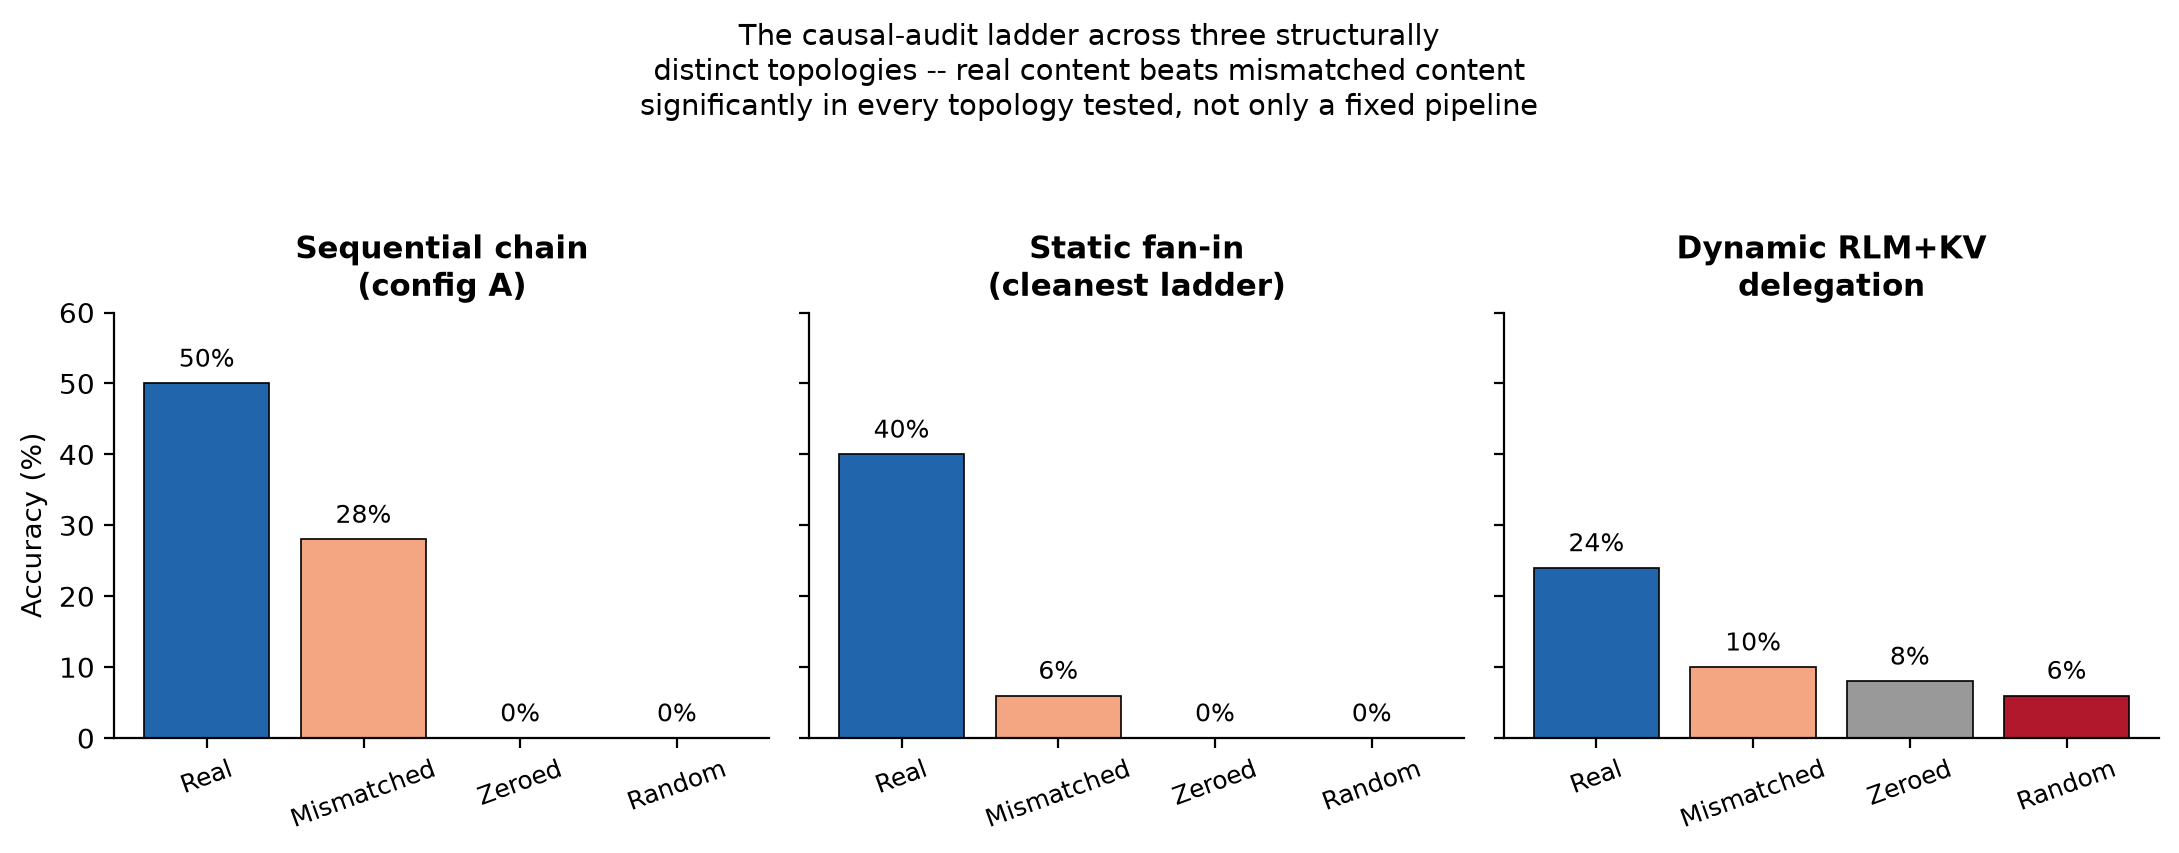
\includegraphics[width=\columnwidth]{figures/fig4_topology_ladder.png}
\caption{The causal-audit ladder across all three topologies. Real
beats mismatched, which beats zeroed/random, in every topology,
including one the model constructs for itself. The recursive
topology's non-zero floor is a discussed scope difference
(\S\ref{sec:method}), not noise.}
\label{fig:topology_ladder}
\end{figure}

\subsection{Topology and architecture dependence}

On Mistral, \texttt{B\_int4\_kivi} and \texttt{B\_int8} replicate the
full ordering, but layer-selection configurations (\texttt{C},
\texttt{D}) show an attenuated pattern: mismatched beats zeroed/random
($p=0.0156$/$0.0078$), but real is not distinguishable from mismatched
($p=0.51$/$0.375$). This tracks \texttt{C}/\texttt{D}'s own degraded
Mistral baseline (20.0\%/22.0\%, well below Qwen's 46.0\%/50.0\%), not
a loss of content-dependence (Appendix~\ref{app:results-ext}). Qwen3-8B
shows a related but distinct pattern, discussed with the dropped
control in \S\ref{sec:results}.1: random still collapses accuracy
($p<0.0001$), but real is not distinguishable from zeroed or mismatched
(all four comparisons $p=0.30$--$0.79$). We verified this is a real
effect, not a bug, via donor-pool leakage checks and selective-overlap
analysis (Appendix~\ref{app:qwen3}).

Fan-in ($n=50$) gives the cleanest, most decisive ordering in our
evaluation: 40.0/53.0 real versus 0.0/0.8 zeroed versus 0.0/0.0 random
versus 6.0/12.0 mismatched. Real vs.\ zeroed/random: $p<0.0001$ each
(F1 delta $+0.522$ [$+0.396,+0.645$] / $+0.530$ [$+0.403,+0.654$]).
Real vs.\ mismatched: $p=0.0001$, 18 of 19 discordant pairs favoring
real (F1 delta $+0.410$ [$+0.267,+0.546$]), the strongest version of
this comparison anywhere in this
paper, because unlike the recursive topology, a corrupted child's
answer has no alternate pathway to route around. Mismatched
vs.\ zeroed/random is underpowered on exact McNemar ($p=0.25$, 3
discordant pairs) but trends real on F1 CI (Appendix
\ref{app:results-ext}).

Layer-selection's accuracy cost differs sharply across the models we
test, though this is three separate single-model comparisons, not a
jointly tested model-by-configuration interaction effect: dropping a
near-identical layer proportion costs 30.5 F1 points on Mistral
($p=0.0001$) but a smaller, not-yet-significant amount on Qwen2.5
($p=0.34$) and Qwen3-8B ($p=1.0$, noise). Incorrect answers
also differ in \emph{kind}, not only rate: Qwen's are short, close
near-misses; Mistral's include fabricated tangents and repetition
loops, not explained by a repetition-penalty confound we checked
directly (Appendix~\ref{app:failurechar}).

\subsection{Model-driven delegation}

The RLM+KV loop (Section~\ref{sec:method}) is deliberately the least
favorable topology for a clean result: our HotpotQA questions do not
need decomposition, and a real REPL loop here solves a harder
coordination problem than the task requires. Consistent with that,
\texttt{kv} versus \texttt{text} accuracy is statistically unresolved
at native scale ($n=50$, 24.0/32.3 vs.\ 22.0/28.5, $p=1.0$); we do not
claim a KV accuracy win, nor that KV is necessary for RLM-style
delegation. The causal audit does resolve: \texttt{kv} vs.\ zeroed
$p=0.0078$ (F1 delta $+0.210$ [$+0.110,+0.323$]), vs.\ random
$p=0.0039$ (F1 delta $+0.230$ [$+0.127,+0.347$]), vs.\ mismatched
$p=0.0156$ (F1 delta $+0.167$ [$+0.071,+0.274$]), the full three-tier
signature on a topology the model constructs for itself. KV remains
causally influential under model-driven delegation even though the
root retains an independent path to the source information; zeroed/
random do not collapse to near-zero here (8.0/6.0 rather than
$\approx$0) because of that independent pathway, a narrower audit than
the fixed topologies' own. A behavioral signal mined from the same
transcripts, whether the model commits to an answer within its turn
budget, tracks the same ordering and resolves the one leg accuracy
alone could not (mismatched vs.\ random, $p<0.0001$; full statistics in
Appendix~\ref{app:behavioral}). An earlier non-determinism in this
prototype's decode loop was diagnosed and fixed; every number above is
confirmed bit-identically reproducible under the fix
(Appendix~\ref{app:nondeterminism}).

Because the root always retains direct access to the original
passages, this native scale is not RLM's own long-input regime
\citep{rlm2026}: at constructed long-context lengths (2,000--16,000
tokens; Appendix~\ref{app:longcontext}) accuracy reverses in
\texttt{text}'s favor and is accompanied by a turn-budget asymmetry
visible directly in the transcripts rather than simple starvation, and
a random-cache-only audit at that scale still separates real
\texttt{kv} from random on whether a session completes at all -- a
narrower claim than the mismatched-inclusive audit above, which we do
not treat as confirming the same content-\emph{specificity} result at
that scale, since no mismatched condition was run there.

\subsection{Implications for KV-cache compression and transformation}

If relay is content-specific, a compressed relay should still show the
same real-versus-mismatched gap as uncompressed relay, not become
generic state merely because it occupies fewer bytes.
Table~\ref{tab:causal_audit_full} already shows \texttt{B\_int8} and
\texttt{B\_int4\_kivi} retain this gap under the zeroed/random/
mismatched ladder on both Qwen2.5 and Mistral: compression does not
turn the cache into interchangeable generic state. We report
compressed bytes and measured single-GPU latency separately
throughout: our evaluation has no network transmission, and a smaller
cache does not measurably speed up our pipeline, since every
transformer layer still runs regardless of injected-cache size
(Limitations).

\begin{table}[t]
\centering
\small
\begin{tabular}{lcc}
\toprule
\textbf{Config} & \textbf{Acc.\ / F1} & \textbf{KV/hop} \\
\midrule
A & 56.0 / 69.1 & 144.35 MB \\
B\_int8 & 57.0 / 70.5 & 72.16 MB (2.00x) \\
B\_int4 & 0.0 / 0.0 & 38.38 MB (4.00x) \\
\textbf{B\_int4\_kivi} & \textbf{52.0 / 64.1} & 36.43 MB (3.96x) \\
C & 43.0 / 57.8 & 104.16 MB \\
D & 50.0 / 61.9 & 37.82 MB (3.82x) \\
E & 9.0 / 17.4 & 35.63 MB \\
\bottomrule
\end{tabular}
\caption{Qwen2.5-7B-Instruct, HotpotQA, $n=100$. Ratios vs.\ A's
144.35~MB. Per-config latency, single-agent/text-agent baselines, and
E\_int8 in Appendix~\ref{app:extratables} (Table~\ref{tab:full}).}
\label{tab:main}
\end{table}

\texttt{A} vs.\ \texttt{B\_int8}: $p=1.0$, 3 discordant examples of 100;
0 on Mistral ($n=50$). This is a genuine, tight near-zero-cost finding,
not an underpowered null. \texttt{B\_int4} (uniform 4-bit, no
per-channel fix) collapsed to 0.0\%/0.0\%, traced to a RoPE/key
interaction (full diagnostic in Appendix~\ref{app:rotation}).
\texttt{B\_int4\_kivi}, a per-channel fix for that interaction,
resolves it at 52.0\%/64.1\% and 3.96x compression with no calibration
profile, showing no detectable difference from \texttt{D} (F1 delta
$+2.2$, 95\% CI $[-8.2, +12.8]$) at higher compression (3.96x
vs.\ 3.82x); it trends below \texttt{A}/\texttt{B\_int8} (52\% vs.\
56--57\%) but this is not yet significant ($p=0.36$--$0.50$; fixing the
value side too does not improve on it further,
Appendix~\ref{app:extratables}). The 3.96x figure is a correction we
report rather than suppress, and its provenance matters: our
compressor initially stored every 4-bit value at a full byte, and
every packed-bits ratio in this paper reflects a packing-enabled
compressor applied \emph{after} the accuracy/F1 numbers above were
measured on the pre-packing version. Packing itself is verified
bit-identical to unpacked output on synthetic tensors, a pure
storage-format change (Appendix~\ref{app:nibble}), but we have not
re-run the full pipeline with packing enabled to directly confirm
accuracy is unaffected end-to-end. An anchor-based offset-correction
mechanism (\texttt{E}) fails outright versus \texttt{D}
($p\approx0.00003$), independent of a decoding confound we ruled out;
full diagnostic in Appendix~\ref{app:limitations}.

\section{Discussion}

The same three-tier ordering holds on every topology we test, but not
with equal strength, and the differences are informative. Fan-in gives
the cleanest signal because a corrupted child's content has no
alternate route to the aggregator; the sequential chain is nearly as
clean; the RLM+KV topology is weakest specifically where the root
retains an independent information pathway, which is a structural
property of that topology, not evidence against the claim. Read
together, these three results suggest non-exchangeability is a
property of relayed content when it is the \emph{only} path to
information, and is naturally harder to detect when a receiver has
another way to get what it needs, exactly as a causal test should
behave.

The Qwen3-8B exception is itself a meta-point: the presence of
content-dependence is not visible from one architecture's behavior
alone, so a compression recipe validated on one model's causal audit is
not safe to assume for another without re-auditing. This is also why we
treat the
compression results as a consequence of the causal findings rather than
an independent contribution: \texttt{B\_int4\_kivi}'s success and
\texttt{E}'s failure are explained by the same structure (RoPE-position
dependence, content-identity dependence) the causal audit already
establishes, not by separate compression-specific reasoning.

\section{Conclusion}

We tested whether a relayed KV cache can be treated as interchangeable
state using a five-condition causal substitution: real, zeroed,
random, mismatched, and dropped. On Qwen2.5-7B-Instruct and
Mistral-7B-Instruct-v0.3, a mismatched cache is worse than both the
correct cache and no cache at all ($p<0.001$ for dropped versus
mismatched on both models), the clearest evidence in this paper that
wrong content is actively harmful, not merely unhelpful. The correct
cache itself is not shown to beat no relay on any model we test in the
chain; we report this as not distinguishable at $n=50$, not as a
finding that the cache is unnecessary. On Qwen3-8B, evaluated in
non-thinking mode, we detect no sensitivity to cache content at all, a
limit we report rather than hide, and one we cannot yet attribute to
architecture, decoding mode, or both. A static fan-in decomposition
shows a different regime from the chain: with no independent copy of
the source passages, the aggregator's correct cache decisively beats a
mismatched one, evidence that the chain's weaker result is tied to
that topology's redundant information path, not a general retraction
of content-dependence. Compressed relays retain the same
real-versus-mismatched gap as uncompressed ones, evidence against
compression silently erasing this dependence, alongside techniques that
fail for reasons this causal framework helps explain
(\S\ref{sec:results}). We adopt, rather than introduce, the
zeroed/random/mismatched methodology \citep{latentcommpay2026}; our
contribution is the dropped control, the two-regime distinction between
chain and fan-in, and evaluating both under compression. We do not
claim these results generalize beyond the models, tasks, and
topologies tested here.

\section{Limitations}
\label{sec:limitations}

\begin{itemize}[leftmargin=*]
\item \textbf{Single-agent accuracy is close to relay accuracy.}
\texttt{single\_agent} (no relay at all) is not clearly separated from
\texttt{A} (the full relay chain) on its own accuracy/F1 either
(Table~\ref{tab:full}, cited and discussed in \S\ref{sec:results});
we did not run a paired test between them specifically.
\item \textbf{Receiver necessity depends on the topology.} Whether the
receiver needs the relayed cache at all is not one answer: the chain
and the fan-in give structurally different dropped-control results for
a stated topological reason (\S\ref{sec:results}), and we do not
average the two into one number.
\item \textbf{A false premise under dropped.} The receiver's own prompt
(Verifier/Finalizer in the chain, the aggregator in the fan-in) asserts
that prior content is already in context; this is false specifically
under dropped (Table~\ref{tab:conditions}). We left prompts identical
across all five conditions so only the cache varies, at the cost of
that one false premise in exactly this condition.
\item \textbf{Qwen3-8B ran in non-thinking mode.} All Qwen3-8B results
use \texttt{enable\_thinking=False}; we did not evaluate thinking mode,
so we cannot separate an architecture effect from a decoding-mode
effect in that model's results.
\item \textbf{Sample size and donor assignment.} Most causal-audit
comparisons in this paper are at $n=50$ (Qwen2.5's chain and fan-in
dropped control are $n=100$, Table~\ref{tab:no_relay}), each with one
donor assignment per example for the mismatched condition, not
resampled across repeated draws; several comparisons remain
underpowered rather than confirmed null even at the larger size
(\S\ref{sec:results}, Appendix~\ref{app:method-ext}).
\item \textbf{2WikiMultihopQA is a confirmation run.} One additional
dataset, one configuration, $n=50$ (Appendix~\ref{app:2wiki}); not a
systematic cross-dataset study.
\item \textbf{Single-process, single-GPU; no latency claim.} No
\texttt{KVMessage} is serialized over a network; compressed-byte
accounting reflects what a distributed deployment would need to send,
not a measured latency speedup, and smaller caches are not observed to
be faster in our setup, since every transformer layer still runs
regardless of injected-cache size (Appendix~\ref{app:limitations}).
\item \textbf{Causal audit coverage.} Covers every relay condition
except \texttt{B\_int4} itself, uninformative to audit given it already
collapses unaudited. The RLM+KV topology's own \texttt{kv}-vs-\texttt{text}
accuracy comparison remains unresolved at native scale; it is resolved,
against \texttt{kv}, only at constructed long-context lengths, a
different regime (\S\ref{sec:results}, Appendix~\ref{app:longcontext}).
\item \textbf{Model and task scope.} Qwen2.5-7B-Instruct and
Mistral-7B-Instruct-v0.3 on the full configuration suite; Qwen3-8B on a
subset. A fourth model family, Phi-3.5-mini-instruct, was dropped after
a pre-existing library/model limitation unrelated to our pipeline
(Appendix~\ref{app:limitations}). Nearly all results are on HotpotQA; one
GSM8K confirmatory run replicated both headline findings. All results
use greedy decoding; we did not evaluate under sampling.
\item \textbf{Cross-architecture relay untested within one pipeline.}
All of our own architecture variation is between separate pipeline
runs, never mixed within one pipeline across agent roles; prior work
reports this can fail outright at the precondition stage for some model
pairings (Appendix~\ref{app:limitations}).
\item \textbf{Statistical power.} Several comparisons are underpowered
rather than confirmed null, notably Qwen2.5's layer-selection cost in
isolation ($\approx$15\% power); our cross-architecture claim rests on
the well-powered Mistral result.
\item \textbf{Bleed-through review.} The donor-content bleed-through
review is a manual, single-annotator, exploratory observation.
\end{itemize}

\bibliography{references_rlm_focus}
\bibliographystyle{acl_natbib}

\appendix

\section{Extended Related Work}
\label{app:relwork}

\paragraph{Rotation-based quantization.}
\label{app:rotation}
We applied a fixed orthonormal
Hadamard rotation to both keys and values before quantizing
(covering PolarQuant's \citep{polarquant2026} rotate-then-quantize
step, not TurboQuant's \citep{turboquant2026} separate QJL
bias-correction term; these are two distinct papers sharing only two
authors, not one work under two names). On our model this produced
severely out-of-distribution decoded output. We traced this to keys'
RoPE encoding: K is cached after RoPE is applied, which mixes channel
pairs by a position-dependent phase, and a second, RoPE-agnostic
rotation disrupts that structure. KIVI \citep{kivi2024} quantizes keys
per-channel and values per-token, motivated by RoPE leaving channel-wise
magnitude more consistent across positions than per-head ranges assume.
RotateKV \citep{rotatekv2025} instead rotates \emph{before} RoPE via
Pre-RoPE Grouped-Head Rotation, explicitly designed to avoid this
interaction. KVQuant \citep{kvquant2024} similarly identifies post-RoPE
key quantization as harder than value quantization for the same reason.

\paragraph{Considered but not adopted compression strategies.}
Orthogonal Backfill \citep{orthobackfill2026} injects a low-rank
residual of discarded content orthogonal to what is retained; its
published formula requires attention weights our \texttt{sdpa} decode
path does not expose, and given our own evidence that naive
reproductions can actively mislead, we did not ship an approximated
version. KVTC \citep{kvtc2026} applies media-compression-style
transform coding (PCA decorrelation, adaptive quantization, entropy
coding) for up to 20x compression, a third paradigm distinct from
uniform quantization and rotation; NVIDIA's kvpress library and
TensorRT-LLM's reuse-aware cache confirm KV compression is an actively
contested axis of deployed systems.

\paragraph{Cheng et al.\ and system-dependence.} Cheng et al.\
\citep{latentcommpay2026} find content-specificity is
\emph{system}-dependent: ceiling effect on LatentMAS, partial on
KVComm, no detected advantage on C2C, holding audit methodology fixed
and varying which published relay system is tested. Our Qwen3-8B
extension independently arrives at the same qualitative pattern while
holding the relay mechanism fixed and varying the model instead. Two
audits converging on ``it depends, and not on accuracy alone'' from
different varied axes is more informative than either alone. ``When KV
Cache Reuse Fails in Multi-Agent Systems'' \citep{kvreusefails2026}
shows reuse strategies effective for generation agents can silently
corrupt an LLM judge's cross-candidate comparison, a complementary
critical-auditing result we do not directly test.

\paragraph{CanonicalMerge.} \citep{canonicalmerge2026} is close to our
fan-in topology: near-identical models (Qwen3-1.7B/4B versus our
Qwen2.5-7B-Instruct/Mistral-7B-Instruct-v0.3) and a closely related task
(HotpotQA bridge questions versus our full distractor HotpotQA),
addressing a real question we do not (whether merge order biases the
result) but reporting only downstream accuracy, with no
causal-intervention test of whether merged content is specifically, not
just numerously, necessary.

\paragraph{AdaK and Pitfalls of KV Cache Compression.} AdaK
\citep{adak2026} reports adaptive KV-budget estimation generalizing
across Qwen3 (4B/8B) and Mistral-7B-Instruct-v0.2, the same two
architecture families we test (not a third; Llama is not among AdaK's
evaluated models despite a superficial reading suggesting otherwise),
which looks like a counterexample to our architecture-dependence claim.
We do not believe it is: AdaK estimates budget per-instance and
per-model at inference time rather than committing to one
calibration-time ranking applied uniformly, so it never assumes a
fixed, transferable ranking is safe to act on; its success is a
positive instance of our principle, not a counterexample. This is our
reading of the mechanism, not a reimplementation we verified ourselves.
``The Pitfalls of KV Cache Compression'' \citep{pitfallskv2026} argues
compression methods optimize aggregate metrics while implicitly
equating token retention with functional preservation; our contribution
is a causally grounded, cross-axis demonstration of this within one
system (depth, position, content-identity) rather than the abstract
observation.

\section{Extended Method}
\label{app:method-ext}

\paragraph{Causal-audit baseline caveat.} Zero-ablation is a
known-imperfect causal baseline in the interpretability literature: it
pushes activations off the training distribution, which can produce
large behavioral changes unrelated to whether the zeroed content
carried meaningful information. We treat moment-matched-random and
mismatched, which preserve realistic statistics or substitute another
real cache, as the more informative evidence, and zero-ablation as a
supplementary sanity floor. A fully rigorous ``no difference'' claim
would use a pre-registered equivalence margin rather than absence of
significance; we did not have the budget to pre-register and power such
a test.

\paragraph{Why RLM+KV is implemented from scratch.} We implement the
RLM+KV loop directly on \texttt{transformers} \citep{transformers2020}
rather than \texttt{dspy.RLM}, the first-party DSPy implementation of
RLM. DSPy is built on \texttt{litellm} and is, by design, a text-only,
API-centric orchestration layer: a sub-call through \texttt{dspy.RLM}'s
\texttt{llm\_query} returns decoded text and nothing else, with no
exposure anywhere in the framework to a model's KV cache. Our
\texttt{kv} return channel is not implementable on top of it; we
verified this against DSPy's own documentation before committing to a
from-scratch implementation.

\section{Extended Results}
\label{app:results-ext}

\paragraph{Qualitative texture (sequential chain).} Mismatched's wrong
answers are coherent and grammatical, real linguistic structure
attached to the wrong question; zeroed produces garbled but
recognizable English; random is more degraded still (code-fragment
tokens, mixed-language noise) despite matching real activation
statistics. We read this as a zero vector being a weak attention key
that can be down-weighted, while realistic random noise resembles
genuine signal and actively misdirects attention. A fan-in
garbage-signature scan of all 200 generations gives the identical
texture: 0/50 flagged for real, 4/50 mismatched, 23/50 zeroed, 48/50
random.

\paragraph{Donor-content bleed-through, in full.} Manually reviewing 20
of 36 incorrect \texttt{A\_audit\_mismatched} answers against their
donor question: one unambiguous instance (a Kansas university
fight-song question produced ``Ellie Goulding,'' traceable only to a
donor question about that singer) and one weaker, ambiguous case; the
remainder show ordinary failure on the real question's own topic. One
annotator, no automated classifier or inter-annotator agreement check;
a rigorous version would classify the full set of incorrect examples
automatically or with multiple annotators, which we did not have the
budget to complete.

\paragraph{Layer-selection cost magnitude, full detail.} The
architecture-dependence claim in Section~\ref{sec:results} compares a
near-identical dropped-layer proportion: 9/32 layers (28\%) on Mistral
versus 8/28 layers (29\%) on Qwen2.5. Mistral's cost (30.5 F1 points,
$p=0.0001$) is confirmed significant; Qwen2.5's smaller cost is not yet
significant at $n=100$ ($p=0.34$), but the cross-model claim does not
rest on that reaching significance: even Qwen's most generous
uncertainty bound (F1 CI upper $+16.4$ points) is under half of
Mistral's confirmed collapse. Qwen3-8B's $D$-vs-$A$ comparison ($p=1.0$)
rests on only 3 discordant pairs out of 50, consistent with noise
rather than a real effect.

\paragraph{Mistral layer-selection, full explanation.} On \texttt{C},
mismatched beats zeroed/random ($p=0.0156$ each) but is not
distinguishable from real ($p=0.51$, F1 CI includes zero); \texttt{D}
shows the identical pattern ($p=0.0078$; $p=0.375$). Both track
\texttt{C}/\texttt{D}'s own degraded Mistral baseline (20.0\%/22.0\%
vs.\ Qwen's 46.0\%/50.0\%): less headroom to detect a further
real-vs-mismatched gap on an already-degraded baseline, not a failure
to replicate content-dependence. \texttt{B\_int8} on Mistral replicates
the full clean pattern, matching every quantization-only configuration;
layer-selection configurations show the attenuated pattern,
quantization-only configurations do not, consistently across two
separate experiments.

\paragraph{GSM8K confirmatory run.} $n=50$, Qwen2.5: \texttt{D} matched
\texttt{A}'s accuracy exactly (McNemar $p=1.0$, more decisively free
than on HotpotQA); the causal audit's three-tier ordering held with
every comparison significant ($p<0.0002$), larger effect sizes than the
original HotpotQA run. One run on one additional task, not a systematic
multi-task study; we did not extend \texttt{B\_int8}/\texttt{D}-family
audits or Mistral to GSM8K.

\paragraph{2WikiMultihopQA confirmatory run, verification detail.}
\label{app:2wiki}
All four conditions (\texttt{A} and its three audit variants) were
scored on the identical 50 paired examples, confirmed by matching
example index, question text, and gold answer across conditions. The
mismatched condition drew from a held-out donor pool of 20 distinct
questions; checking every donor question against all 50 scored
questions directly, none matched, and all 100 mismatched substitutions
(50 examples times two relay hops) were confirmed applied via the
per-example audit logs. Accuracy, F1, and latency were independently
reconstructed from the per-example records and matched the evaluator's
own summary exactly. Real versus mismatched had 19 discordant pairs,
all 19 favoring real and none favoring mismatched, F1 delta $+39.1$
points, 95\% bootstrap CI $[+26.1, +52.3]$. This is a single
confirmatory run on one additional dataset and one configuration, not a
systematic cross-dataset study.

\paragraph{Fan-in mismatched-vs-zeroed/random leg.} Not significant by
exact McNemar ($p=0.25$ each, 3 discordant pairs, the test's own floor
at that count), but the F1 bootstrap CI excludes zero for both
($+0.112$ [$+0.035,+0.200$], $+0.120$ [$+0.047,+0.206$]):
accuracy-level evidence is underpowered at this $n$ for this specific
leg while the finer-grained F1 comparison trends real.

\section{Qwen3-8B Verification}
\label{app:qwen3}

We verified the Qwen3-8B exception (Section~\ref{sec:results}) is a
real effect, not a bug, three ways: no donor-question pool leakage;
\texttt{A\_audit\_zeroed} and \texttt{D\_audit\_zeroed} produce
byte-identical output on all 50 examples, which looked alarming until
traced to \texttt{D}'s own \texttt{zeros} reconstruction strategy
composing correctly with the audit's own zeroing, not a bug; and real,
zeroed, and mismatched overlap on only 10--24 of 50 examples pairwise,
confirming the substitution takes effect selectively rather than being
silently inert. We do not have a mechanistic explanation for the
difference; we report it as an empirical observation and flag candidate
mechanisms as future work.

\section{RLM+KV Behavioral Signal}
\label{app:behavioral}

Timeout rate, mean turn count, and mean delegation-call count are
monotonic across conditions (real 22\% timeout, 7.72 turns, 1.38 calls;
mismatched 42\%/8.48/1.12; zeroed 72\%/9.46/0.76; random 76\%/9.60/0.66).
Substituting ``session finished without exhausting its turn budget''
for ``correct'' in the same paired McNemar test, every comparison is
significant, including mismatched versus random ($p<0.0001$), exactly
the leg final-answer accuracy left unresolved (real vs.\ mismatched
$p=0.0309$; real vs.\ zeroed/random $p<0.0001$ each; mismatched vs.\
zeroed $p=0.0001$). We verified this run shows no new degenerate output
at this scale (0/50 flagged for real/text; a clean, monotonic
3/50--48/50 ordering across the remaining conditions).

\section{RLM+KV Non-Determinism: Diagnosis and Fix}
\label{app:nondeterminism}

An earlier run of this experiment was not run-to-run deterministic.
Diffing raw generations for the identical 50 questions between two
independent runs under greedy decoding found 15 of 50 (30\%)
\texttt{text}-channel examples produced genuinely different output,
plausibly GPU floating-point non-associativity cascading through this
prototype's long, self-referential decode loop (unlike the two fixed
topologies, confirmed bit-identical across reruns). We fixed this by
forcing \texttt{torch.use\_deterministic\_algorithms(True,
warn\_only=True)} and setting \texttt{CUBLAS\_WORKSPACE\_CONFIG} before
any CUDA context exists. Verification: a rerun of the \texttt{text}
channel on 20 questions produced 0/20 differing raw answers against the
pre-fix run, including all 7 of the originally divergent examples. We
then reran the full five-channel, $n=50$ ladder and diffed every field,
not only the ones reported in Section~\ref{sec:results}: exact match,
F1, timeout rate, and delegation-call count are bit-identical across
both runs (0 of 250 raw answers differ). One harmless nuance: 33 of the
\texttt{random} condition's 50 examples show different intermediate
turn-by-turn wording despite both independently exhausting their turn
budget on the identical question with the identical final outcome; this
never affects any scored quantity in this paper.

Separately, getting a working baseline for this topology at all
required diagnosing and fixing three real engineering failure modes: a
sub-call's own prompt framing leaking into the receiver's attention
when spliced without isolating the generated answer span; a
session-wide repetition-tracking loss specific to a persistent,
turn-continuing cache; and a RoPE position-shift bug specific to
splicing an answer-only, prompt-truncated child KV, verified two ways
(a corrected unit test and a real-model rerun showing every previously
degenerate example become coherent).

\section{RLM+KV Long-Context Stress Test}
\label{app:longcontext}

We tested the RLM+KV topology at constructed long-context lengths
(2,000 and 16,000 tokens), built by combining each question's real
HotpotQA passages with filler drawn from a disjoint pool of other
questions, grown to a target token count and shuffled together. This
is a deliberately constructed stress-test regime, not a naturally
occurring long-context task, built specifically to probe the context
lengths RLM's own motivating regime targets rather than HotpotQA's
native scale.

\paragraph{Accuracy comparison.} At both lengths ($n=25$ each),
\texttt{text} wins every discordant pair against \texttt{kv} (10 of
10 total), the reverse of the near-parity native-scale result in
Section~\ref{sec:results}.

\paragraph{Ruling out batch dilution.} We tested whether \texttt{kv}'s
disadvantage stems from its uncompressed splice diluting relevant
signal across a large delegated batch, by comparing delegation batch
sizes of 20 and 3 at the 16,000-token length. \texttt{kv}'s own
accuracy is identical (8.0\%) regardless of batch size across two
independent samples (pooled $n=50$), and \texttt{text} continues to
win more discordant pairs at the smaller batch size as well (McNemar
$p=0.34$ pooled, F1 CI [$-0.227$, $+0.039$]): directionally
consistent, not formally significant, but sufficient to rule out
within-batch signal dilution as the explanation.

\paragraph{Turn-budget asymmetry.} Substituting ``finished within its
turn budget'' for ``correct'' in the same paired McNemar test used
throughout this paper: at batch size 20 ($n=25$), $p=0.0005$, 12 of 12
discordant pairs favor \texttt{text} finishing; at batch size 3
(pooled $n=50$), $p<0.000001$, 32 of 33 discordant pairs favor
\texttt{text}. \texttt{kv}'s mean delegation-call count grows sharply
as batch size shrinks (3.76 at batch size 20 to 13.24 and 21.04 at
batch size 3 across the two samples) while \texttt{text}'s stays flat
(approximately 2.4 to 2.7): smaller batches redistribute \texttt{kv}'s
work into more rounds it cannot complete in time, rather than reducing
the total work. Doubling the turn budget (40 to 80, $n=15$) does not
resolve this: \texttt{kv}'s timeout rate is unchanged (53\% versus 52
to 76\% across configurations), ruling out simple turn-budget
starvation as the explanation.

\paragraph{Native-scale latency.} The same mechanism produces a
measurable latency cost at native scale even though \texttt{kv} does
not lose there on accuracy: 11.4s versus 9.6s mean wall-clock time per
example ($n=50$), despite splicing only a short, cheap answer span.
The gap decomposes into more timeouts (22\% versus 14\%, and a
timed-out session costs 2 to 3 times a finished one) and, even
restricted to sessions that finish within budget, more root turns
(6.79 versus 5.95) and more delegation calls (1.38 versus 1.14) before
committing to an answer, not a cost in the splice operation itself.

\paragraph{Causal audit at long context.} Substituting real \texttt{kv}
with random content collapses the delegated-and-completed rate
decisively at this scale ($n=30$, $p<0.0001$, 18 of 18 discordant
pairs favoring real content). This is a real-versus-random result
only; no mismatched condition was run at this scale, so we do not read
it as confirming the content-\emph{specificity} claim of
Section~\ref{sec:results}, only that real content still beats pure
noise at this scale.

\section{Fan-in Causal Audit: Design Bug and Fix}
\label{app:faninbug}

An early version substituted only one of two children's KV by default,
leaving the other's real content as an unaudited shortcut. This
produced a near-null pilot result (3/10 exact-match for real versus
3/10 for zeroed) that, on inspection, was a weaker test than intended:
5 of 10 zeroed-condition outputs already showed the expected
garbled-output signature, meaning the aggregator was still succeeding
on the uncorrupted child often enough to mask the effect. We fixed this
by substituting every child's KV (extracted into a directly testable
helper function with its own unit tests), matching the full-relay-
corruption strength of the sequential pipeline's own audit. The
corrected result is the one reported in Section~\ref{sec:results}.

\section{Nibble-Packing: Byte-Accounting Bug and Real Fix}
\label{app:nibble}

Our compressor initially stored every quantized tensor as one full
\texttt{torch.uint8} per element regardless of bit-width, so a 4-bit
value took the same byte an 8-bit value did; first-reported compression
ratios assumed packing that did not exist. We implemented genuine
two-values-per-byte packing (pack after quantizing for \texttt{bits==4},
unpack before dequantizing), verified via unit tests covering
round-trip exactness (including odd-length/padding edge cases,
full-nibble-range coverage) and, most directly, bit-identical
\texttt{compress}/\texttt{decompress} output with and without packing,
confirming packing is a pure storage-format change. The corrected
ratios land back at almost exactly the originally reported figures: the
original formula's arithmetic (0.5 bytes/element for 4-bit) was always
what real packing would produce; the bug was that nothing in the
compressor actually packed anything. This is unit-tested at the tensor
level, not confirmed via a live GPU rerun of the full pipeline with
packing enabled; reported accuracy/F1 figures come from pre-packing
runs, only compression-ratio figures reflect the packing-enabled
compressor.

\section{Layer-Selection Failure Character: Full Statistics}
\label{app:failurechar}

Qwen's incorrect \texttt{D} answers average 18 characters, 2\%
exceeding 150, overwhelmingly close near-misses (reformatted dates,
dropped honorifics, single-character typos). Mistral's average 109
characters, 15\% exceeding 150, maximum 1,454, including fluent
fabricated tangents (e.g.\ a full invented biography of an unrelated
person) and degenerate repetition loops essentially absent from Qwen's
failure set. We checked the obvious confound, that our fixed
repetition penalty under-penalizes Mistral relative to its own tuned
defaults, against each model's published \texttt{generation\_config.json}:
Qwen's own default is exactly our setting (1.05); Mistral's specifies
none, so our setting applies \emph{more} correction for Mistral, the
opposite of what the confound needs. The long-tail pattern persists
anyway.

\section{Additional Configurations and Tables}
\label{app:extratables}

Table~\ref{tab:full} reports every configuration's latency alongside
accuracy/F1/KV-per-hop, the full version of Table~\ref{tab:main}
including the two no-relay controls and \texttt{E\_int8}. We report
compressed bytes and latency as two distinct quantities throughout this
paper (Section~\ref{sec:results}): our evaluation has no network
transmission, and a smaller cache does not measurably speed up our
single-GPU pipeline.

\begin{table}[h]
\centering
\small
\begin{tabular}{lcccc}
\toprule
\textbf{Config} & \textbf{Acc.} & \textbf{F1} & \textbf{Lat.} & \textbf{KV/hop} \\
\midrule
single\_agent & 57.0 & 68.4 & 1.6s & --- \\
text\_agent & 54.0 & 68.3 & 7.2s & --- \\
A & 56.0 & 69.1 & 8.6s & 144.35 MB \\
B\_int8 & 57.0 & 70.5 & 8.3s & 72.16 MB \\
B\_int4 & 0.0 & 0.0 & 39.4s & 38.38 MB \\
B\_int4\_kivi & 52.0 & 64.1 & 9.6s & 36.43 MB \\
C & 43.0 & 57.8 & 10.0s & 104.16 MB \\
D & 50.0 & 61.9 & 10.2s & 37.82 MB \\
E & 9.0 & 17.4 & 19.8s & 35.63 MB \\
E\_int8 & 1.0 & 6.2 & 22.2s & 49.05 MB \\
\bottomrule
\end{tabular}
\caption{Full version of Table~\ref{tab:main} (Qwen2.5-7B-Instruct,
HotpotQA, $n=100$), with latency and the no-relay controls.}
\label{tab:full}
\end{table}

\texttt{single\_agent} and \texttt{text\_agent} are no-KV-relay
controls: every KV-relay configuration shares identical prompts with
\texttt{text\_agent}, so accuracy/latency deltas are attributable to
the relay mechanism itself. \texttt{E\_int8} (uniform-int8 variant of
the offset-correction baseline) also fails catastrophically, consistent
with Section~\ref{sec:results}'s \texttt{E} result. Fixing KIVI's value side
too (\texttt{B\_int4\_kivi\_full}, per-token quantization) does not
improve on \texttt{B\_int4\_kivi} (44.0\% vs.\ 50.0\% on a matched
50-example subset, $p=0.51$, trending the other way) and is worse on
compression (3.75x vs.\ 3.99x self-referential): per-token quantization
stores a scale/zero-point pair per sequence position, and sequence
length vastly exceeds K's per-channel grouping (128 channels). Together
with an earlier null result for rotating values instead, two
independently motivated value-side interventions both failed, evidence
the key/RoPE interaction was \texttt{B\_int4}'s entire failure
mechanism, not one of several factors.

\section{Scope and Engineering Detail}
\label{app:limitations}
% Retitled from "Extended Limitations": the paper now has exactly one
% section titled "Limitations" (main text, before this appendix). This
% section holds the supporting detail and numbers that section points
% to, per the ARR instruction to keep Limitations itself qualitative.

\paragraph{Single-process, single-GPU.} Every experiment runs within
one Python process on one RTX 4090; compression-ratio and
transmitted-byte accounting reflects what a real distributed deployment
would need to send, but latency numbers exclude network transfer, and
smaller relayed caches are not observed to be faster, since the model
executes every transformer layer regardless of injected-cache contents.
A systems-scale deployment study (multi-GPU, real network transfer,
concurrent load) was out of scope.

\paragraph{Recursive topology engineering.} Even with the fixes in
Appendix~\ref{app:nondeterminism}, the \texttt{kv}-versus-\texttt{text}
accuracy comparison remains genuinely unresolved at native scale
($n=50$), not merely underpowered in a way we expect more data to
trivially resolve. At constructed long-context lengths this comparison
is resolved, against \texttt{kv} (Appendix~\ref{app:longcontext}), a
regime boundary on efficiency that does not extend to the causal
content-dependence result, which still holds there. Beyond the three
topologies tested here, a genuinely adversarial fan-in
topology \citep{latentagentslie2026} and LatentMAS's layer-wise KV
concatenation \citep{latentmas2026} remain untested against our
specific methodology.

\paragraph{Scope detail.} Phi-3.5-mini-instruct was dropped after two
real bugs were fixed in how our pipeline hands decode off to
\texttt{model.generate()} under non-default RoPE scaling, yet the model
still failed past roughly 4{,}096 tokens, its own
\texttt{original\_max\_position\_embeddings}; plain, unmodified
\texttt{model.generate()} with no pipeline code involved degrades
identically past the same threshold, isolating this to a pre-existing
model/library limitation, not our pipeline. HotpotQA's per-hop contexts
(1{,}500--2{,}500+ tokens) routinely push our relay chain's cumulative
cache past this threshold, ruling the model out regardless of further
fixes. One further methodological risk: Cheng et al.\
\citep{latentcommpay2026} report at least one model pairing where the
receiver could not consume a relayed cache at all, i.e.\
cross-architecture relay can fail at the precondition stage; all of our
own architecture variation is between pipeline runs, not within one
pipeline mixing architectures across agent roles, which remains, to our
knowledge, an open problem in this literature (KVCOMM itself flags it as
future work). All results use greedy decoding; we did not evaluate
under sampling or self-consistency.

\paragraph{Offset-correction task scope.} KVCOMM was evaluated on MMLU,
GSM8K, and HumanEval, none of which is multi-hop QA; whether the
technique fares differently on the more homogeneous task family it was
validated on remains open (our GSM8K check did not re-test \texttt{E}).

\paragraph{Partial reproduction.} Our rotation-based quantization omits
TurboQuant's QJL bias-correction term; our KIVI-inspired fix omits the
original method's group-wise windowing and fp16 residual buffer. Both
are inspired-by implementations scoped to test a specific hypothesis,
not certified reproductions.

We checked ARR's guidance on whether a separate Ethical Considerations
section was warranted: this work uses two long-established public
benchmarks, two openly released model checkpoints, no human subjects,
no crowdsourcing, and no new data collection; we are not aware of a
concern beyond what this section already covers.

\end{document}
